\quad 1.\quad Установка git, nodejs, npm и grunt.
\newline Для установки всего необходимого, нам нужно открыть терминал, нажав на его иконку. 

\begin{figure}[h]
		\centering
		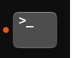
\includegraphics[width=0.2\linewidth]{VM/5.png}
\caption{Терминал.}
\label{ris:image}
\end{figure}

\quad Далее, для скачивания, необходимо ввести соответствующие строки кода:
\newline \texttt{git – sudo apt install git}
\newline \texttt{nodejs – sudo apt install nodejs}
\newline \texttt{npm - sudo apt install npm}
\newline \texttt{grunt - sudo apt install grunt}
\newline Чтобы удостовериться, что всё правильно скачалось, можно узнать версию данного продукта. Например: \texttt{git –version}

\quad 2.\quad  Регистрация на GitHub.
\newline \quad Для регистрации на GitHub нужно перейти по ссылке: : https://github.com/ и заполнить всю необходимую информацию о себе.

\quad     3. \quad Работа с репозиторием.
\newline \quad Переходим по ссылке: https://github.com/nickkolok/chas-ege/. Далее нажимаем на зелёную кнопку с надписью «Code», и копируем ссылку репозитория. Лучше сделать это сразу, потому что Ubuntu на VirtualBox может сильно нагружать компьютер, и открыть вкладку с браузером может быть проблематично из-за нагрузки. (Если возникли проблемы с копирование ссылки, то можно открыть браузер внутри Ubuntu, перейти по ссылке и скопировать ссылку репозитория в нём.)

\begin{figure}[h]
		\centering
		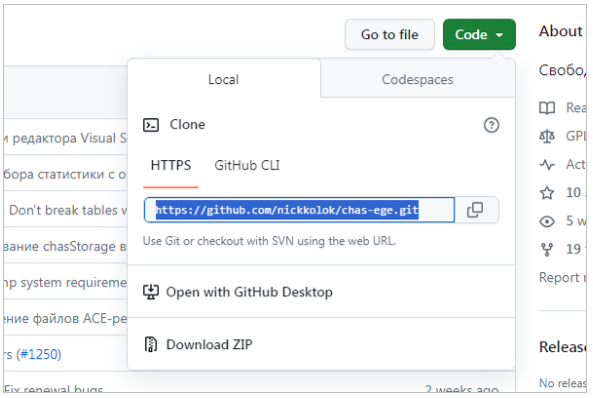
\includegraphics[width=0.9\linewidth]{VM/6.png}
\caption{Github. Ссылка на репозиторий.}
\label{ris:image}
\end{figure}

• Далее снова заходим в терминал и создаём папку на рабочем столе командой: mkdir <название папки>. Можно убедиться, что папка создана, с помощью команды: ls. Мы увидим все папки на рабочем столе, среди которых должна быть только что созданная.Затем заходим в папку командой: cd <название папки>, и клонируем себе репозиторий командой: git clone <ссылка на репозиторий >

• Добавляем себе ссылку на основной репозиторий проекта с помощью команды: git remote add upstream <ссылка на репозиторий> и убеждаемся, что он подключился, командой: git fetch upstream 

• Собираем проект командой: grunt. Важно выполнять эту команду в папке, в которую мы и склонировали репозиторий.

• Открываем файл dist/sh/otladka.html в браузере командой: «open otladka.html», и запускаем любой шаблон, для проверки, в открывшемся окне.


\begin{figure}[h]
		\centering
		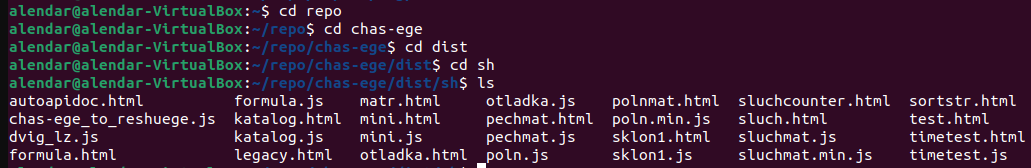
\includegraphics[width=1\linewidth]{VM/7.png}
\caption{Путь к файлу otladka.html.}
\label{ris:image}
\end{figure}

4.\quad  Создание SSH ключа для возможности подключиться к удалённому репозиторию.
Для начала нужно проверить наличие ключа, введя следующие команды:
\newline \texttt{cd ~/.ssh}
\newline \texttt{ls}

Если файлов с названиями \texttt{id\_dsa} и \texttt{id\_dsa.pub} нет (открытый и приватный ключ), то можно создать их используя команду:
\newline  \texttt{ssh-keygen -o}
\newline \quad Далее нужно открыть содержимое файла dsa.pub командой:
\newline  \texttt{cat ~/.ssh/ id\_dsa.pub}

Далее добавили свой ключ себе в аккаунт на GitHub, чтобы иметь возможность подключиться к удалённому репозиторию. А также прописали ещё одну команду, необходимую для подключения.

\begin{figure}[h]
		\centering
		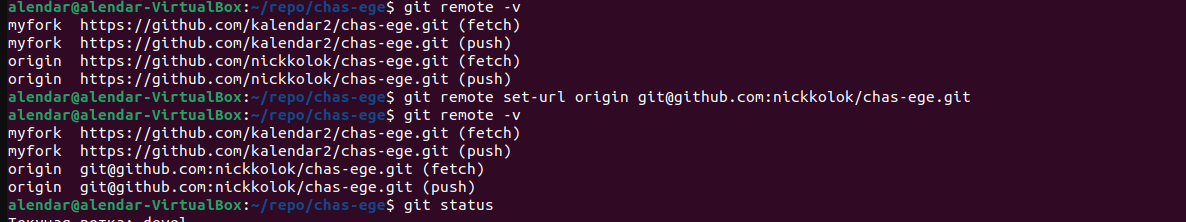
\includegraphics[width=1\linewidth]{VM/pod.png}
\caption{Подключению к удалённому репозиторию с помощью команды.}
\label{ris:image}
\end{figure}

Перейдя в репозиторий на GitHub «ЧАС-ЕГЭ», нужно нажать кнопку «Fork» справа вверху.

Открыв VirtualBox и войдя в свою виртуальную машину, открыли терминал и перешли в папку с «Час ЕГЭ» с помошью команды cd git/chas-ege.

Представление гиту выглядит следующим образом:
\newline \texttt{git config --global user.name «Фамилия Имя»}
\newline \texttt{git config --global user.email «электронная почта пользователя»}
\newline Можно придать выводу гита красные и зелёные цвета с помощью команд:
\texttt{git config --global color.ui true}
\newline Добавление своего форка на гитхаб в список удалённых репозиториев:
\texttt{git remote add myfork git@ github.com:«GitHubNik»/chas-ege.git}, где «GitHubNik» - ник пользователя на гитхабе. 

Основные команды для создания и отправления изменений в удалённый репозиторий:
\\Переключение на основную ветку (devel):
\\ \texttt{git checkout devel}
\\ \quad Её обновление (В некоторых случаях применима также команда: \texttt{git pull origin devel}):
\\ \texttt{git fetch origin devel}
\\ \quad Создание новой ветки:
\\ \texttt{git checkout -b newtask-777}
\\ \quad Проверка изменений, а также самой ветки:
\\ \texttt{git status}
\\ \quad Добавление всех изменений:
\\ \texttt{git add .}
\\ \quad Добавление всех изменений:
\\ \texttt{git commit -m «Внесены изменения в файл ...»}
\\ \quad Отправка изменений в удалённый репозиторий:
\\ \texttt{git push myfork newtask-777:myfork newtask-777:}

5.\quad  Игнорирование ненужных файлов и каталогов.

Для того, чтобы сообщить Git, какие файлы или каталоги нужно игнорировать , можно создать .gitignore файл.

Для этого необходимо открыть Терминал и перейти к расположению репозитория Git. Далее создаётся файл для репозитория, с помощью команды \texttt{touch .gitignore}.

Если файл уже был отправлен в репозиторий, необходимо отменить отслеживание файла, прежде чем добавлено правило игнорирования, с помощью команды: \texttt{git rm --cached FILENAME}.

Файл не видим, как и все файлы с точкой в начале названия файла, но его можно увидеть с помощью команды \texttt{ls -a}. Зайдя в него, нужно записать путь к файлу или каталогу, который будет игнорироваться.

\begin{figure}[h]
		\centering
		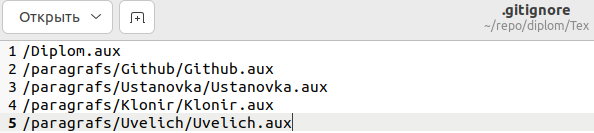
\includegraphics[width=0.6\linewidth]{VM/gitignore.png}
\caption{Файл .gitignore с списком файлов для игнорирования в нём.}
\label{ris:image}
\end{figure}

Это не единственный способ задания игнорирования файла или каталога. Можно также сообщить Git всегда игнорировать определенные файлы во всех репозиториях на компьютере. Для этого, например, каталог нужно добавить в файл с именем ignore , расположенным внутри каталога \texttt{~/.config/git}.

Также можно вообще не создавать файл .gitignore. Этот метод можно использовать для локально создаваемых файлов, которые не должны создавать другие пользователи. Для этого, используя текстовый редактор, нужно открыть файл, вызываемый \texttt{.git/info/exclude} в корневом каталоге репозитория Git.